\documentclass{beamer}
\usepackage{graphicx}
\usepackage{PaloAlto}
\usepackage{tikz}

\title{Presentation on Turing award winner}
\subtitle{Raj Reddy :The 28th Turing awardee}
\author{P.Anurag}
\institute{SCIS University of Hyderabad}
\date{September 13, 2017}


\begin{document}
%\setbackgroundtemplate{%
%\tikz\node[opacity=0.5]
 %{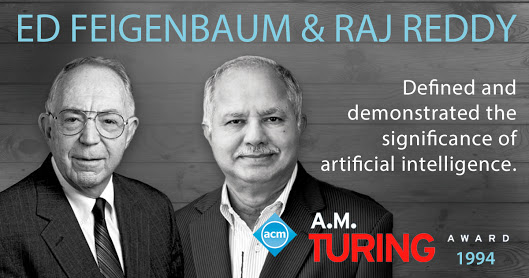
\includegraphics[width=\paperwidth,height=\paperheight]{rajco.jpg}};}
 
 \maketitle
 
\begin{frame}

\begin{figure}
 \centering
 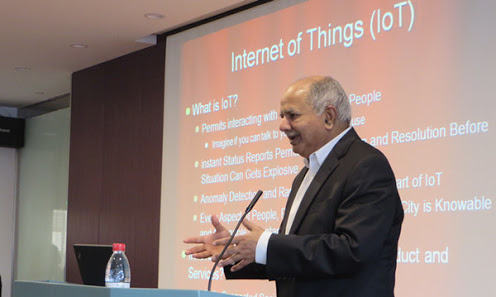
\includegraphics[scale=0.5]{raj1.jpg}
\end{figure} 


\begin{block}{}
 Raj Reddy Professor of Computer science and Robotics at carnegie mellon University
\end{block}

\end{frame}

 
\begin{frame}
  \frametitle{Table of contents}
  \begin{enumerate}
   \item 
  \end{enumerate}

\end{frame}

\begin{frame}
 \frametitle{\bf Qualifications}
  \begin{block}
    \begin{tabular}{cccc}
     {\bf Degree} & {\bf Specilization} & {\bf Year} & {\bf institute} \\
     Bachelor of science & civil engneering & 1958 & University of Madras (now {\bf Anna University}) \\
     Master of science & Information Technology & 1960 & University of new south wales \\
     Doctrate & Computer Science & 1966 & Stanford university \\
    \end{tabular}

  \end{block}
\end{frame}




\end{document}



